\section{Laser}
Ein Laser besteht prinzipiell aus 3 Bestandteilen: dem laseraktiven Medium, der Pumpe und dem Resonator.\\
Bevor die Funktionsweise des Lasers beschrieben werden kann, müssen vorher einige Begriffe geklärt werden:
\subsection{Absorption, spontane und induzierte Emission, Besetzungsinversion}
Wird ein Atom im Grundzustand $E_1$ in ein Strahlungsfeld gebracht, so kann es durch beispielsweise \textbf{Absorption} 
eines Photons Energie aufnehmen und somit in einen angeregten Zustand $E_2$ übergehen. Das Photon muss mindestens eine 
Energie von $E_p = h \nu = E_2 - E_1$ besitzen, diese wird dem Strahlungsfeld entzogen.\\
Dieser angeregte Zustand $E_2$ möchte wieder in den Grundzustand $E_1$ zurück, da dieser der energetisch günstigere (niedrigere) Zustand ist, dies kann auf zwei verschiedene Emissionsarten geschehen:\\
Bei der \textbf{spontanen Emission} sendet der angeregte Zustand $E_2$  ein Photon aus. Der Übergang vom angeregten Zustand $E_2$ in den Grundzustand $E_1$ findet hier ohne äußere Einwirkung eines zusätzlichen Feldes statt. Dieser Vorgang passiert spontan, d.h. der Prozess geschieht zufällig und folgt somit statistischen Gesetzen. \\
Die zweite Möglichkeit ist die sogenannte \textbf{stimulierte oder induzierte Emission}. 
Befindet sich ein Atom oder Molekül in einem angeregtem Zustand $E_2$, in einem geeigneten Strahlungsfeld, so ist 
es möglich, dass ein Photon diesen angeregten Zustand trifft, noch bevor dieser spontan emittieren kann. 
Wenn dies der Fall ist, dann ist bei dem angeregten Zustand keine Absorption des Photons mehr möglich und 
so kommt es zur Emission eines weiteren Photons. Der angeregte Zustand fällt zurück in einen 
niedrigeren Zustand, meist den Grundzustand $E_1$ zurück. 
Wenn die beide Photonen die gleiche Energie, Schwingungsphase, Bewegungsrichtung und Polarisation haben,
nennt man sie auch \textit{kohärente Photonen}. Kohärente Photonen führen zu einer Verstärkung des 
Strahlungsfeldes. \\
Das folgende Bild zeigt noch einmal den schematischen Ablauf der oben aufgeführten Prozesse:
\begin{figure}[h]
    \centering
    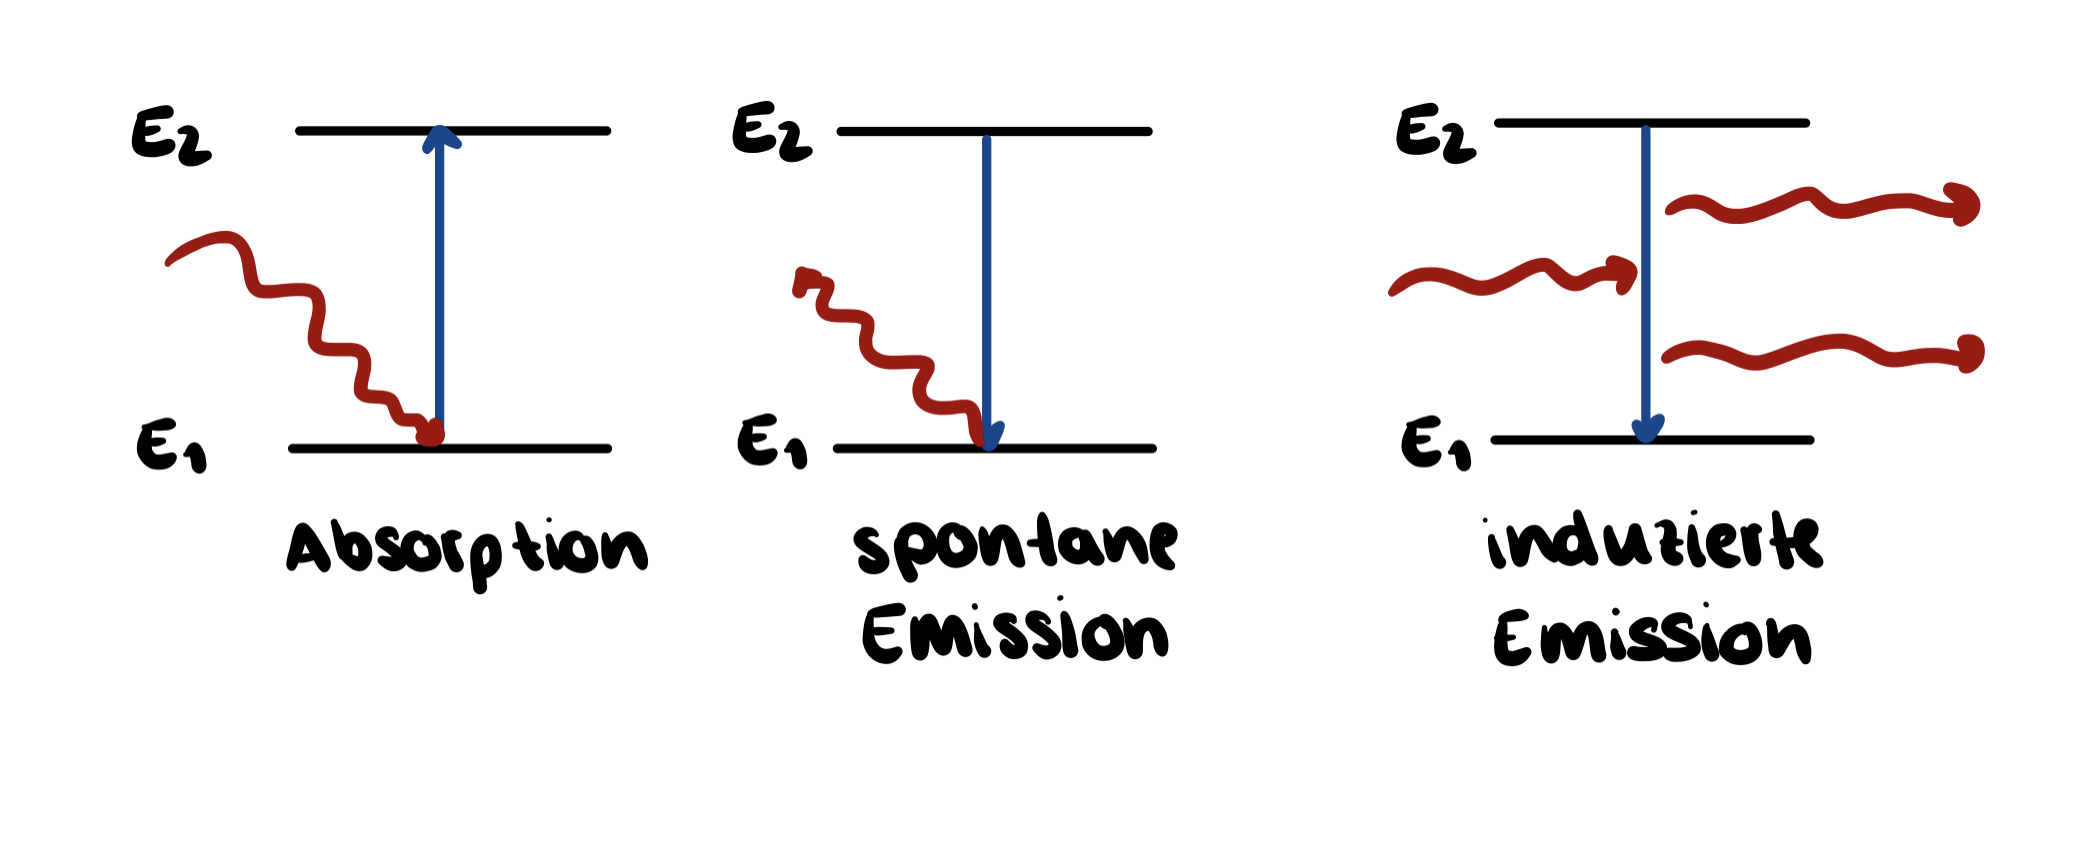
\includegraphics[scale=0.17]{Bilder/FzV/Emission.jpg}
    \caption{Schematische Darstellung von Absorption, spontaner und stimulierter Emission}
\end{figure}
\newpage
Die Wahrscheinlichkeit dieser Emissionsformen und der Absorption können mithilfe der Einstein-Koeffizienten berechnet werden.\\ 
In einem physikalischen System ist es wahrscheinlicher, dass die Besetzungsanzahl des Grundzustandes höher ist, als die Anzahl an 
besetzen angeregten Zuständen. Ist dies jedoch umgekehrt, d.h. wenn sich mehr Teilchen in einem angeregtem bzw. 
energetisch höheren Zustand $E_2$ befinden als in einem energetisch niedrigeren Zustand (Grundzustand), 
spricht man von einer \textbf{Besetzungsinversion}. \cite[vgl.][]{laser1,laser2}


\subsection{Lasermedium}
Das Lasermedium ist entscheidend für die Eigenschaften des Lasers. Es gibt unterschiedliche laseraktive Medien, 
einige Beispiele sind Gase, Kristalle oder Dioden.
In unserem Versuch ist es ein Helium-Neon-Gas, es handelt 
sich hier also um einen Gaslaser.\\
Damit ein Laser funktionieren kann, muss das laseraktive Medium einige theoretische
Voraussetzungen erfüllen. Eine Voraussetzung ist, dass es möglich sein 
muss, dass sich im Medium eine Besetzungsinversion einstellen kann.
Dies ist nicht möglich bei einem Zwei-Niveau-System ($E_1$, $E_2$), das heißt man benötigt ein 3- bzw. 4-Niveau System, dies wird im Folgenden noch einmal diskutiert werden.\\
Mithilfe der Pumpe wird Energie in das laseraktive Medium 'gepumpt' und somit die Zustände im Medium angeregt. 
Das führt dazu, dass im laseraktiven Medium die Photonen spontan emittieren.
Diese freiwerdenden Photonen
treffen auf weitere angeregte Zustände, es kommt zur stimulierten Emission. Durch 
das Aussenden eines weiteren Photons, welches auch noch die gleiche Bewegungsrichtung hat, kommt es zur Verstärkung des 
Strahlungsfeldes und somit wirkt das Lasermedium wie ein optischer 
Lichtverstärker. Durch die richtigen Abmessungen des Resonators, hat das Photon die Möglichkeit das Laseraktive Medium
mehrfach zu durchlaufen, somit kommt es auch zu einer höheren Anzahl an induzierter Emission. \citep[vgl.][]{laser}


\subsection{Pumpe}
Mithilfe der Pumpe wird Energie dem Lasermedium zugeführt.
Diese 'Pumpenergie' ist wichtig, damit sich die Besetzungsinversion einstellen kann. 
Durch diese Energie werden die Atome und Moleküle im Lasermedium in angeregte Zustände versetzt. \\
Man unterscheidet zwischen einer optischen Pumpe, hierbei wird Licht eingestrahlt, und einer elektrischen Pumpe. 
In unserem Fall wird eine elektrische Pumpe verwendet, hier kommt es mithilfe 
von Gasentladung zu einer Energiezufuhr.\\
Das Wichtige an der Pumpleistung ist, dass sie groß genug sein muss, um die Zahl der durch stimulierte Emission über der Zahl der absorbierten Teilchen zu halten. \citep[vgl.][]{laser1, laser2}


\subsection{Resonator}
Der Laserresonator besteht aus einem Spiegelsystem oder/und anderen optischen Elementen.\\
Im Regelfall besteht er aus zwei sich gegenüberliegenden parallelen Spiegeln. Der eine Spiegel sollte 
beinahe total reflektierend sein, in unserem Fall zu 99,9\% und der zweite sollte noch 
ein gewisses Maß an Transmission (hier: 98\% Reflexion) haben, damit der Laserstrahl auch ausgesendet werden kann.
Die Spiegel sorgen dafür, dass die Strahlung durch ein Gebiet, indem Besetzungsinversion vorherrscht, geleitet wird. 
Durch die richtige Anordnung der Spiegel ist es möglich, dass die entstehende Welle das Medium mehrmals durchlaufen kann, dies erhöht wiederrum
Wahrscheinlichkeit der stimulierten Emission, es kommt also zu einer Verstärkung des Lasers. \citep[vgl.][]{laser1}\\
In unserem Versuch besteht der Laserresonator aus zwei sphärischen Spiegeln. Ein Vorteil von sphärischen Spiegeln ist, 
dass sie leicht verkippte Strahlen wieder auf die optische Achse zurück reflektieren können, somit ist der Laserstrahl stabiler. Es muss noch eine weitere Bedingung erfüllt sein damit ein Laser stabil läuft:
\begin{equation}
    0 \leq g_1 \cdot g_2 \leq 1
\end{equation} 
wobei für die Apparaturkonstanten $g_i$ gilt:
\begin{equation}
    g_i = 1 - \frac{L}{r_i}
\end{equation}
$L$ steht für die Länge des Resonators und $r_i$ für den Krümmungsradius des jeweiligen Spiegels. \\
Zusätzlich handelt es sich bei unserer Spiegelanordnung um eine konfokale Anordnung. 
Dies ist ein Spezialfall, hierbei ist Länge des Resonators gleich dem Krümmungsradius. 
Dies hat zur Folge, dass der Strahl den Resonator, im Idealfall, viermal durchläuft. 
Es kommt also zu einer weiteren Verlängerung des Laserstrahls und somit zu einer erhöhten Wahrscheinlichkeit der stimulierten Emission. \citep[vgl.][]{laser}
\begin{figure}[h]
    \centering
    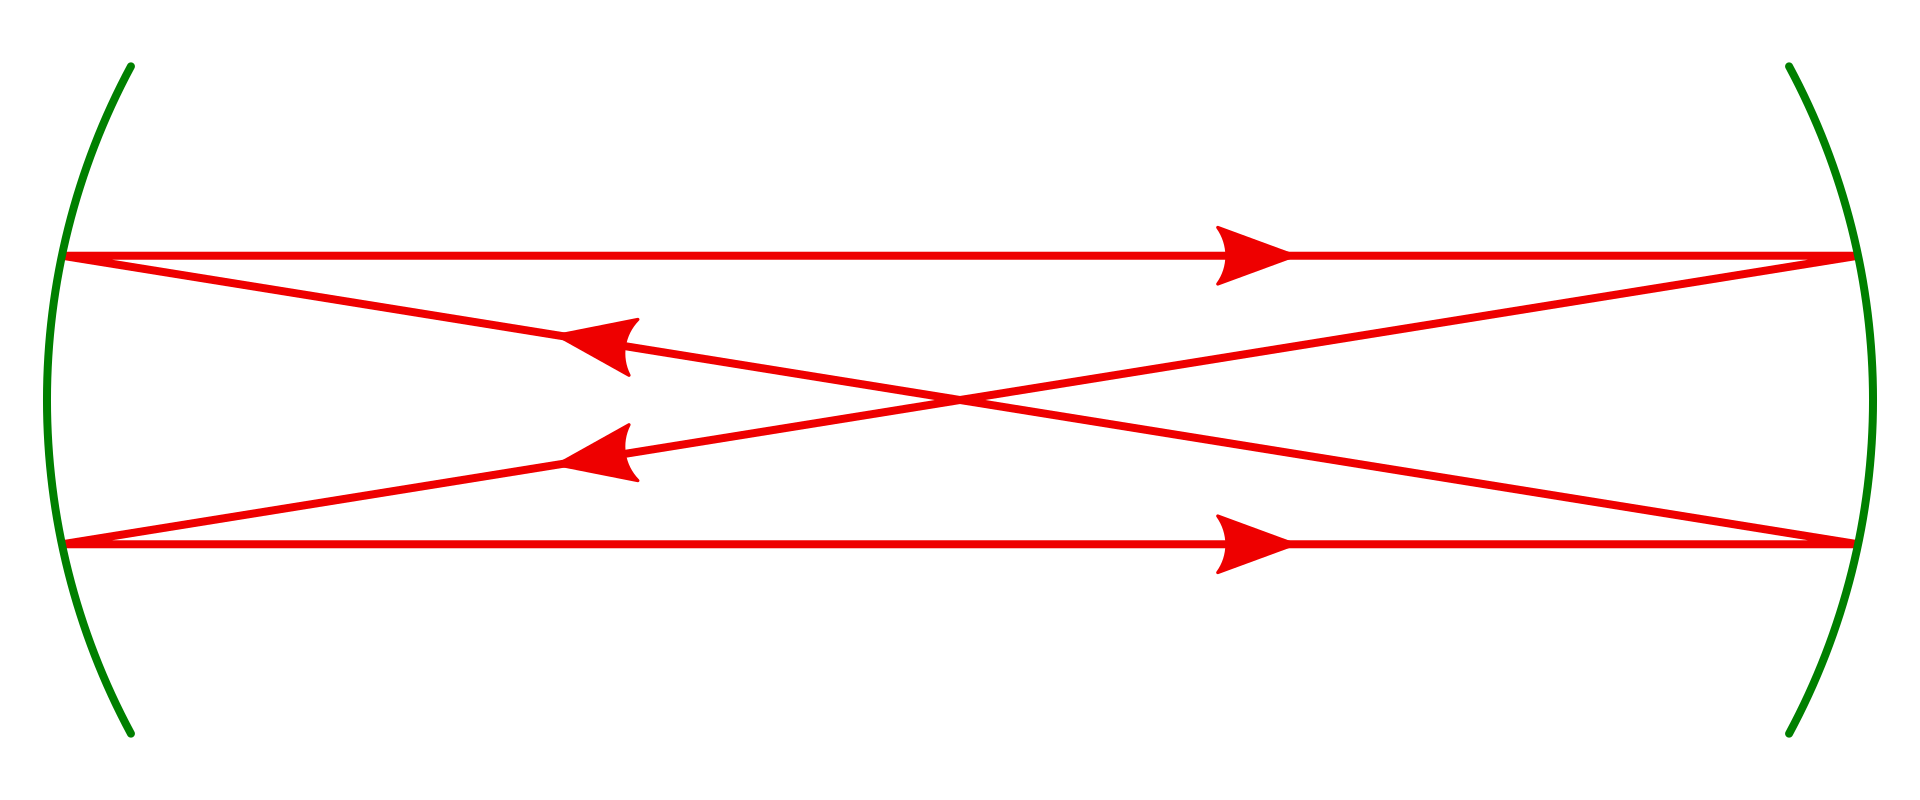
\includegraphics[scale=0.13]{Bilder/FzV/konfokale.png}
    \caption{Darstellung des Strahlenverlauf in einem konfokalen Resonator.}
\end{figure}


\subsection{He-Ne-Laser}
Bei einem Helium-Neon Laser wird als Pumpenergie elektrische Energie verwendet. Durch eine 
Hochspannungsquelle und Elektroden kommt es zu einer Gasentladung in der Glasröhre, also dem Laseraktiven Medium. 
Die Atome, vor allem die Helium-Atome, werden durch die Energie der Stöße mit den frei beweglichen Elektronen angeregt.
Diese angeregten Heliumatome stoßen ihrerseits mit den Neon-Atomen zusammen und regen diese somit an. 
Somit folgt eine Besetzungsinversion bei den Neon-Atomen.\\ 
Das Termschema eines He-Ne-Lasers soll im Folgenden genauer betrachtet werden:
\begin{figure}[h]
    \centering
    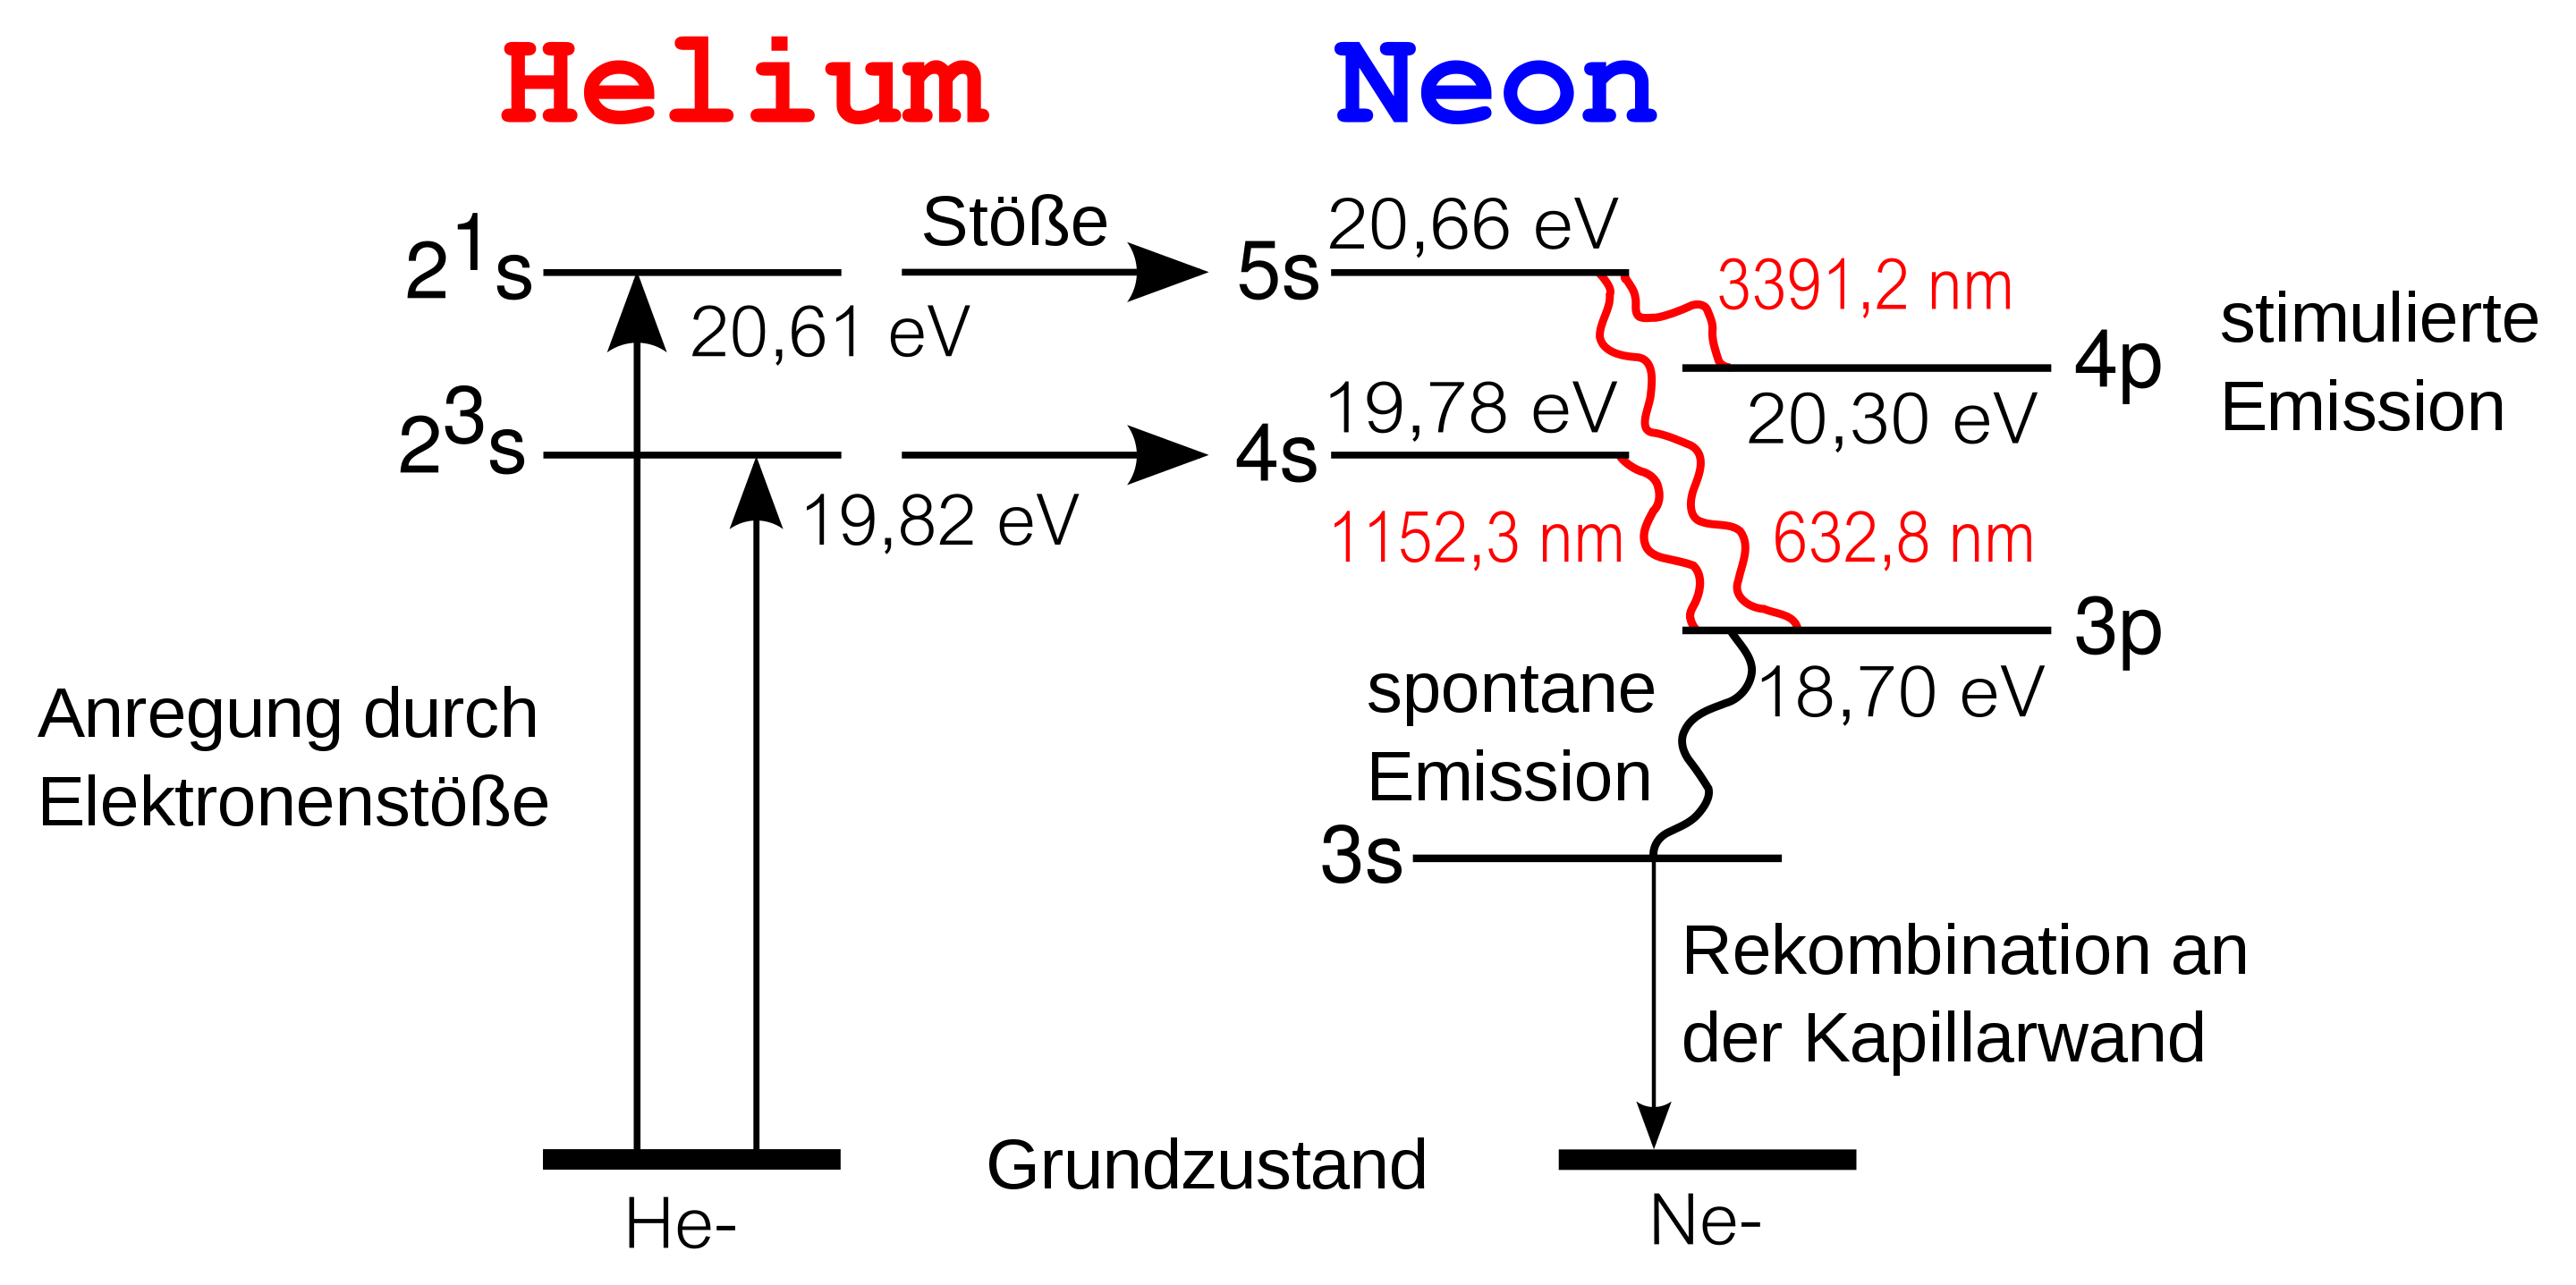
\includegraphics[width=0.6\textwidth]{FzV/TermschemaHeNe.png}
    \caption{Termschema eines Helium-Neon-Laser.}
    \label{fig:Termschema}
\end{figure}\\
Wie aus der vorangegangen Abbildung \ref{fig:Termschema} ersichtlich findet der Laserübergang
im Neon statt. Allerdings benötigt man das Helium, damit die Besetzungsinversion erreicht werden kann, wie oben bereits geschildert. 
Nun gibt es drei mögliche Übergänge im Neon: $5s$ zu $4p$, von $5s$ nach $3p$ und $4s$ nach $3p$. 
Der Laserübergang ist hierbei der Übergang von $5s$ zu $3p$, mit einer Wellenlänge von 632,8\,nm, im sichtbaren Bereich.
Die beiden anderen Übergänge werden mithilfe der sphärischen Spiegel nicht weiter beachtet. \citep[vgl.][]{henelaser}


\subsection{Drei- und Vierniveaulaser}
Wie bereits erwähnt muss ein Laseraktives Medium eine Besetzungsinversion ausbilden können.
Um diese Besetzungsinversion zu erreichen, muss die Lebensdauer der angeregten Zustände verlängert werden. 
Dies ist möglich, indem man weitere Energieniveaus hinzufügt.\\
Über dem $E_2$ wird noch ein weiterer Zustand $E_3$ hinzugefügt. 
Die Anregung erfolgt von $E_1$ auf das angeregte Niveau $E_3$. Anschließend
relaxieren sie strahlungslos in den metastabilen Zustand $E_2$. 
Dieser hat eine relativ lange Lebensdauer (metastabil) und somit kann die 
Besetzungsinversion erreicht werden, da viele Atome in den $E_2$ Zustand
gelangen. Der eigentliche Laserübergang findet dann vom Niveau $E_2$ zu $E_1$ statt. 
Die Lebensdauer ist deutlich höher als bei einem Zwei-Niveau-Laser, das hat den
Vorteil, dass das Atom vermehrt durch stimulierte Emission abgeregt wird.
Der Vierniveaulaser hat zusätzlich noch ein viertes Niveau $E_4$. 
Die Anregung findet nun von $E_1$ auf $E_4$ statt, anschließend kommt es wieder zu einem strahlungslosen
Übergang in den metastabilen Zustand $E_3$. 
Der Laserübergang findet nun zwischen dem Niveau $E_3$ und $E_2$ statt. 
Das hat zur Folge, dass das 'neue' Niveau frei ist und wieder
aufnahmefähig ist, obwohl der Grundzustand $E_1$ nicht leer ist, somit kommt es zu einer
höhere Besetzungsinversion. Der Zustand $E_2$ kann wieder in den Grundzustand $E_1$ zurückkehren. \citep[vgl.][]{laser3}\\
Im Folgenden ist eine schematische Abbildung dieser Niveaus zu sehen:\\
\begin{figure}[h]
    \centering
    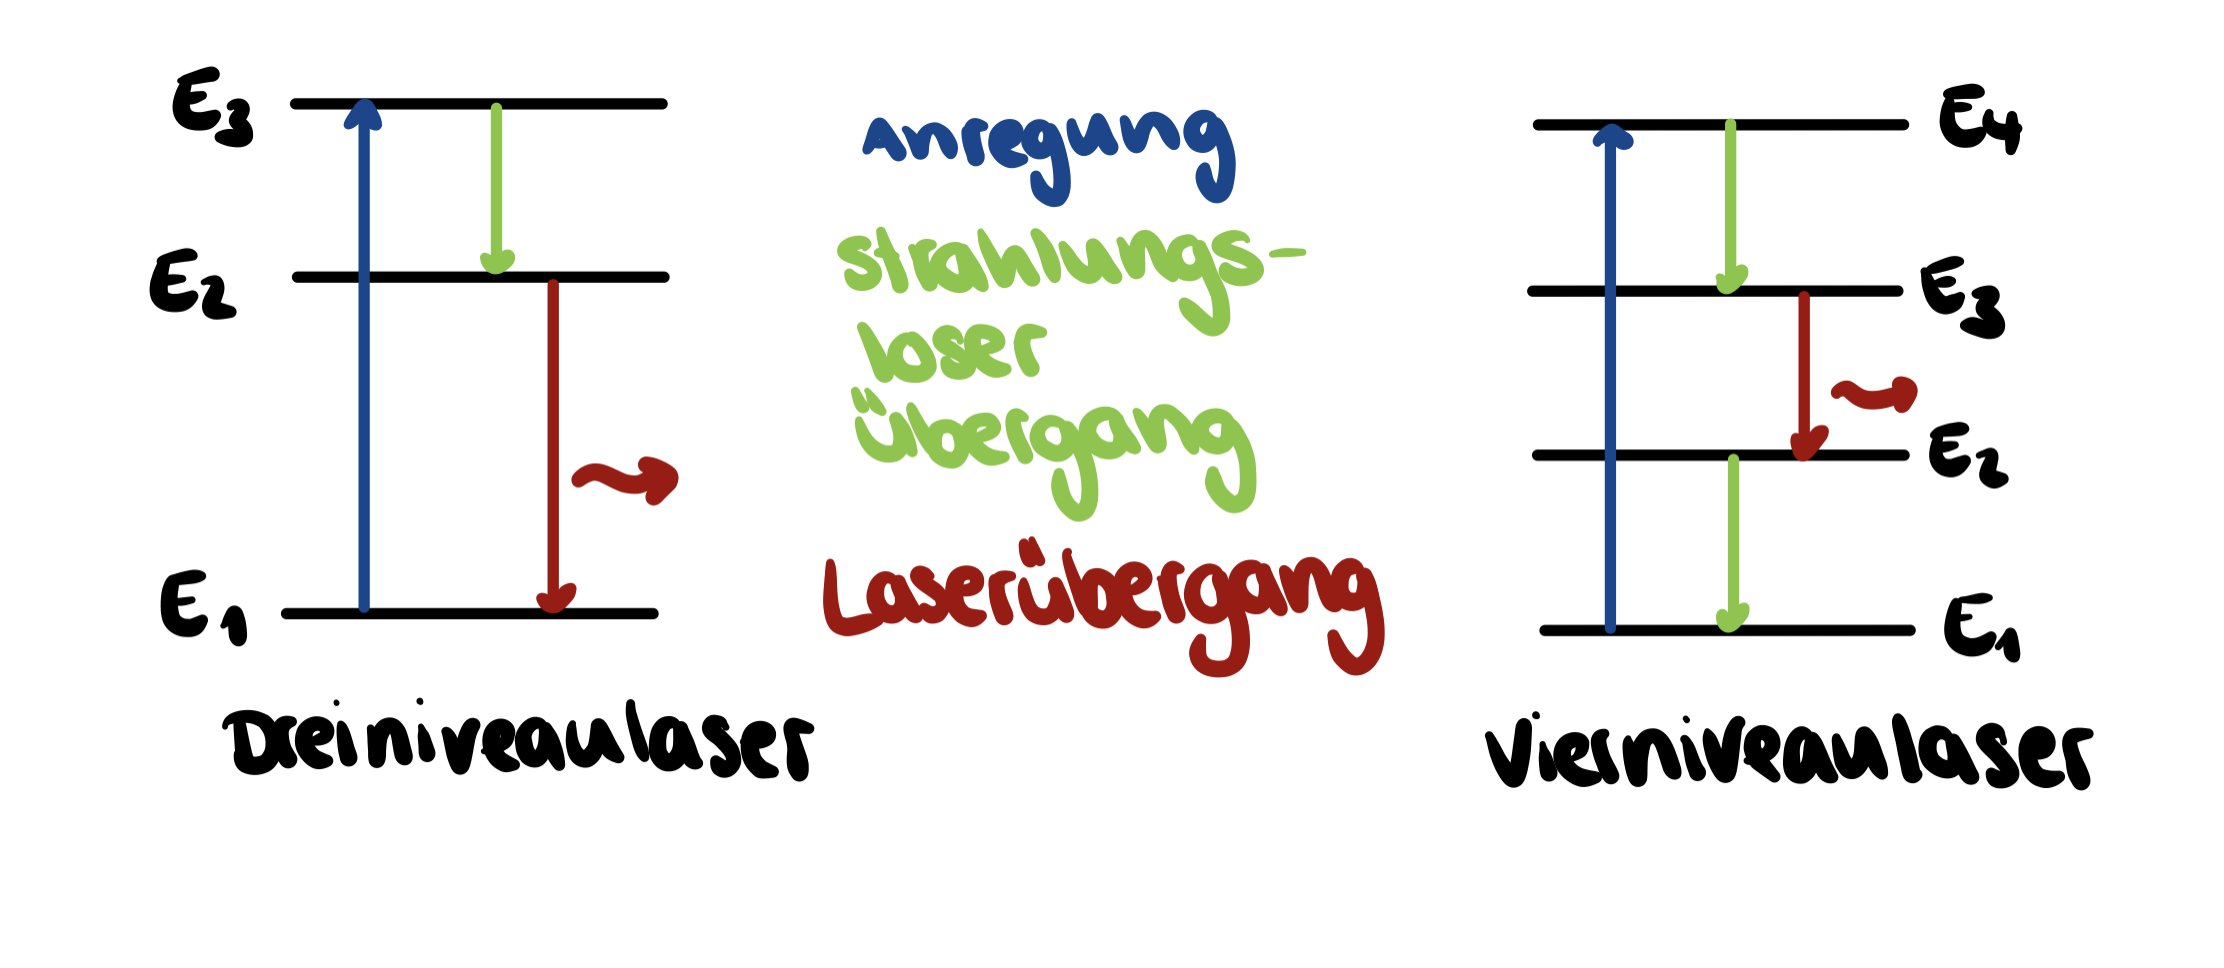
\includegraphics[scale=0.13]{Bilder/FzV/34Niveau.jpeg}
    \caption{Darstellung der Energieniveaus eines Drei- und Vierniveaulaser.}
\end{figure}



